\documentclass{article}
\usepackage{amsmath}
\usepackage{fullpage}
\usepackage{pgfplots}
\usepackage[aux]{rerunfilecheck}
\usepackage{tikz}
\usetikzlibrary{calc}

\newcommand{\ds}{\displaystyle}

% Macros for MATH 110 course dates

\newcommand{\commonTheme}{metropolis}
\newcommand{\commonColorTheme}{metropolis}

\newcommand{\commonAuthor}{Edward Doolittle}
\newcommand{\commonInstitute}{Department of Indigenous Knowledge and
  Science \\ First Nations University of Canada}
\newcommand{\commonCourse}{MATH 110 Calculus I}
\newcommand{\commonTerm}{202510}
\newcommand{\commonDate}{January 6, 2025}

% Review Material

% Lab 0
\newcommand{\commonEventNegativeOne}{LabNegativeOne}
\newcommand{\commonDateLabNegativeOne}{Monday, January 6, 2025}
\newcommand{\commonTitleLabNegativeOne}{MATH 110 Lab 0}
\newcommand{\commonSubtitleLabNegativeOne}{No Lab; Course Opens}

% Section 001
\newcommand{\commonEventZeroZeroOne}{ZeroZeroOne}
\newcommand{\commonDateZeroZeroOne}{Tuesday, January 7, 2025}
\newcommand{\commonTitleZeroZeroOne}{MATH 110 Review 0.1}
\newcommand{\commonSubtitleZeroZeroOne}{Review of Algebra}
\newcommand{\commonPSTitleZeroZeroOne}{MATH 110 Review Problem Set 0.1}

% Section 00A
\newcommand{\commonEventZeroZeroA}{ZeroZeroA}
\newcommand{\commonDateZeroZeroA}{Tuesday, January 7, 2025}
\newcommand{\commonTitleZeroZeroA}{MATH 110 Review 0.A}
\newcommand{\commonSubtitleZeroZeroA}{Review of Inequalities and
  Absolute Values}
\newcommand{\commonPSTitleZeroZeroA}{MATH 110 Review Problem Set 0.A}

% Section 00B
\newcommand{\commonEventZeroZeroB}{ZeroZeroB}
\newcommand{\commonDateZeroZeroB}{Tuesday, January 7, 2025}
\newcommand{\commonTitleZeroZeroB}{MATH 110 Review 0.B}
\newcommand{\commonSubtitleZeroZeroB}{Review of Coordinate Geometry
  and Lines}
\newcommand{\commonPSTitleZeroZeroB}{MATH 110 Review Problem Set 0.B}

% Section 00C
\newcommand{\commonEventZeroZeroC}{ZeroZeroC}
\newcommand{\commonDateZeroZeroC}{Thursday, January 9, 2025}
\newcommand{\commonTitleZeroZeroC}{MATH 110 Review 0.C}
\newcommand{\commonSubtitleZeroZeroC}{Review of Graphs of Second
  Degree Equations}
\newcommand{\commonPSTitleZeroZeroC}{MATH 110 Review Problem Set 0.C}

% Section 00D
\newcommand{\commonEventZeroZeroD}{ZeroZeroD}
\newcommand{\commonDateZeroZeroD}{Thursday, January 9, 2025}
\newcommand{\commonTitleZeroZeroD}{MATH 110 Review 0.D}
\newcommand{\commonSubtitleZeroZeroD}{Review of Trigonometry}
\newcommand{\commonPSTitleZeroZeroD}{MATH 110 Review Problem Set 0.D}

% Section 011
\newcommand{\commonEventZeroOneOne}{ZeroOneOne}
\newcommand{\commonDateZeroOneOne}{Thursday, January 9, 2025}
\newcommand{\commonTitleZeroOneOne}{MATH 110 Review 1.1}
\newcommand{\commonSubtitleZeroOneOne}{Review of Functions}
\newcommand{\commonPSTitleZeroOneOne}{MATH 110 Review Problem Set 1.1}


% Main Course

% Lab 1
\newcommand{\commonEventZero}{LabZero}
\newcommand{\commonDateLabZero}{Monday, January 13, 2025}
\newcommand{\commonTitleLabZero}{MATH 110 Lab 1}
\newcommand{\commonSubtitleLabZero}{Quiz 0: STACK, Onboarding}

% Section 1.4
\newcommand{\commonEventOne}{ZeroOneFour}
\newcommand{\commonDateZeroOneFour}{Tuesday, January 14, 2025}
\newcommand{\commonTitleZeroOneFour}{MATH 110 Lecture 1.4}
\newcommand{\commonSubtitleZeroOneFour}{The Tangent and Velocity Problems}
\newcommand{\commonPSTitleZeroOneFour}{MATH 110 Problem Set 1.4}

% Section 1.5
\newcommand{\commonEventTwo}{ZeroOneFive}
\newcommand{\commonDateZeroOneFive}{Thursday, January 16, 2025}
\newcommand{\commonTitleZeroOneFive}{MATH 110 Lecture 1.5}
\newcommand{\commonSubtitleZeroOneFive}{The Limit of a Function}
\newcommand{\commonPSTitleZeroOneFive}{MATH 110 Problem Set 1.5}

% Lab 2
\newcommand{\commonEventThree}{LabOne}
\newcommand{\commonDateLabOne}{Monday, January 20, 2025}
\newcommand{\commonTitleLabOne}{MATH 110 Lab 2}
\newcommand{\commonSubtitleLabOne}{Quiz 1: Review}

% Section 1.6
\newcommand{\commonEventFour}{ZeroOneSix}
\newcommand{\commonDateZeroOneSix}{Tuesday, January 21, 2025}
\newcommand{\commonTitleZeroOneSix}{MATH 110 Lecture 1.6}
\newcommand{\commonSubtitleZeroOneSix}{Calculating Limits Using the Limit Laws}
\newcommand{\commonPSTitleZeroOneSix}{MATH 110 Problem Set 1.6}

% Section 1.7
\newcommand{\commonEventFive}{ZeroOneSeven}
\newcommand{\commonDateZeroOneSeven}{(Not covered)}
\newcommand{\commonTitleZeroOneSeven}{MATH 110 Lecture 1.7}
\newcommand{\commonSubtitleZeroOneSeven}{The Precise Definition of a Limit}
\newcommand{\commonPSTitleZeroOneSeven}{MATH 110 Problem Set 1.7}

% Section 1.8
\newcommand{\commonEventSix}{ZeroOneEight}
\newcommand{\commonDateZeroOneEight}{Thursday, January 23, 2025}
\newcommand{\commonTitleZeroOneEight}{MATH 110 Lecture 1.8}
\newcommand{\commonSubtitleZeroOneEight}{Continuity}
\newcommand{\commonPSTitleZeroOneEight}{MATH 110 Problem Set 1.8}

% Lab 3
\newcommand{\commonEventSeven}{LabTwo}
\newcommand{\commonDateLabTwo}{Monday, January 27, 2025}
\newcommand{\commonTitleLabTwo}{MATH 110 Lab 3}
\newcommand{\commonSubtitleLabTwo}{Quiz 2: Sections 1.4, 1.5}

% Section 2.1
\newcommand{\commonEventEight}{ZeroTwoOne}
\newcommand{\commonDateZeroTwoOne}{Tuesday, January 28, 2025}
\newcommand{\commonTitleZeroTwoOne}{MATH 110 Lecture 2.1}
\newcommand{\commonSubtitleZeroTwoOne}{Derivatives and Rates of Change}
\newcommand{\commonPSTitleZeroTwoOne}{MATH 110 Problem Set 2.1}

% Section 2.2
\newcommand{\commonEventNine}{ZeroTwoTwo}
\newcommand{\commonDateZeroTwoTwo}{Thursday, January 30, 2025}
\newcommand{\commonTitleZeroTwoTwo}{MATH 110 Lecture 2.2}
\newcommand{\commonSubtitleZeroTwoTwo}{The Derivative as a Function}
\newcommand{\commonPSTitleZeroTwoTwo}{MATH 110 Problem Set 2.2}

% Lab 4
\newcommand{\commonEventTen}{LabThree}
\newcommand{\commonDateMTOne}{Monday, February 3, 2025} 
\newcommand{\commonDateLabThree}{Monday, February 3, 2025}
\newcommand{\commonTitleLabThree}{MATH 110 Lab 4}
\newcommand{\commonSubtitleLabThree}{Midterm: Review, Chapter 1}

% Section 2.3
\newcommand{\commonEventEleven}{ZeroTwoThree}
\newcommand{\commonDateZeroTwoThree}{Tuesday, February 4, 2025}
\newcommand{\commonTitleZeroTwoThree}{MATH 110 Lecture 2.3}
\newcommand{\commonSubtitleZeroTwoThree}{Differentiation Formulas}
\newcommand{\commonPSTitleZeroTwoThree}{MATH 110 Problem Set 2.3}

% Section 2.4
\newcommand{\commonEventTwelve}{ZeroTwoFour}
\newcommand{\commonDateZeroTwoFour}{Thursday, February 6, 2025}
\newcommand{\commonTitleZeroTwoFour}{MATH 110 Lecture 2.4}
\newcommand{\commonSubtitleZeroTwoFour}{Derivatives of Trigonometric Functions}
\newcommand{\commonPSTitleZeroTwoFour}{MATH 110 Problem Set 2.4}

% Lab 5
\newcommand{\commonEventThirteen}{LabFour}
\newcommand{\commonDateLabFour}{Monday, February 10, 2025}
\newcommand{\commonTitleLabFour}{MATH 110 Lab 5}
\newcommand{\commonSubtitleLabFour}{Quiz 3: Sections 2.1, 2.2}

% Section 2.5
\newcommand{\commonEventFourteen}{ZeroTwoFive}
\newcommand{\commonDateZeroTwoFive}{Tuesday, February 11, 2025}
\newcommand{\commonTitleZeroTwoFive}{MATH 110 Lecture 2.5}
\newcommand{\commonSubtitleZeroTwoFive}{The Chain Rule}
\newcommand{\commonPSTitleZeroTwoFive}{MATH 110 Problem Set 2.5}

% Section 2.6
\newcommand{\commonEventFifteen}{ZeroTwoSix}
\newcommand{\commonDateZeroTwoSix}{Thursday, February 13, 2025}
\newcommand{\commonTitleZeroTwoSix}{MATH 110 Lecture 2.6}
\newcommand{\commonSubtitleZeroTwoSix}{Implicit Differentiation}
\newcommand{\commonPSTitleZeroTwoSix}{MATH 110 Problem Set 2.6}

% Lab 6
\newcommand{\commonEventSixteen}{LabFive}
\newcommand{\commonDateLabFive}{Monday, February 24, 2025}
\newcommand{\commonTitleLabFive}{MATH 110 Lab 6}
\newcommand{\commonSubtitleLabFive}{Quiz 4: Sections 2.3, 2.4}

% Section 2.7
\newcommand{\commonEventSeventeen}{ZeroTwoSeven}
\newcommand{\commonDateZeroTwoSeven}{Tuesday, February 25, 2025}
\newcommand{\commonTitleZeroTwoSeven}{MATH 110 Lecture 2.7}
\newcommand{\commonSubtitleZeroTwoSeven}{Rates of Change in the
  Natural and Social Sciences}
\newcommand{\commonPSTitleZeroTwoSeven}{MATH 110 Problem Set 2.7}

% Section 2.8
\newcommand{\commonEventEighteen}{ZeroTwoEight}
\newcommand{\commonDateZeroTwoEight}{Thursday, February 27, 2025}
\newcommand{\commonTitleZeroTwoEight}{MATH 110 Lecture 2.8}
\newcommand{\commonSubtitleZeroTwoEight}{Related Rates}
\newcommand{\commonPSTitleZeroTwoEight}{MATH 110 Problem Set 2.8}

% Lab 7
\newcommand{\commonEventNineteen}{LabSix}
\newcommand{\commonDateLabSix}{Monday, March 3, 2025}
\newcommand{\commonTitleLabSix}{MATH 110 Lab 7}
\newcommand{\commonSubtitleLabSix}{Quiz 5: Sections 2.5, 2.6}

% Section 3.1
\newcommand{\commonEventTwenty}{ZeroThreeOne}
\newcommand{\commonDateZeroThreeOne}{Tuesday, March 4, 2025}
\newcommand{\commonTitleZeroThreeOne}{MATH 110 Lecture 3.1}
\newcommand{\commonSubtitleZeroThreeOne}{Maximum and Minimum Values}
\newcommand{\commonPSTitleZeroThreeOne}{MATH 11 Problem Set 3.1}

% Section 3.2
\newcommand{\commonEventTwentyOne}{ZeroThreeTwo}
\newcommand{\commonDateZeroThreeTwo}{Thursday, March 6, 2025}
\newcommand{\commonTitleZeroThreeTwo}{MATH 110 Lecture 3.2}
\newcommand{\commonSubtitleZeroThreeTwo}{The Mean Value Theorem}
\newcommand{\commonPSTitleZeroThreeTwo}{MATH 110 Problem Set 3.2}

% Lab 8
\newcommand{\commonEventTwentyTwo}{LabSeven}
\newcommand{\commonDateMTTwo}{Monday, March 10, 2025}
\newcommand{\commonDateLabSeven}{Monday, March 10, 2025}
\newcommand{\commonTitleLabSeven}{MATH 110 Lab 8}
\newcommand{\commonSubtitleLabSeven}{Midterm: Chapter 2}

% Section 3.3
\newcommand{\commonEventTwentyThree}{ZeroThreeThree}
\newcommand{\commonDateZeroThreeThree}{Tuesday, March 11, 2025}
\newcommand{\commonTitleZeroThreeThree}{MATH 110 Lecture 3.3}
\newcommand{\commonSubtitleZeroThreeThree}{How Derivatives Affect the
  Shape of a Graph}
\newcommand{\commonPSTitleZeroThreeThree}{MATH 110 Problem Set 3.3}

% Section 3.4
\newcommand{\commonEventTwentyFour}{ZeroThreeFour}
\newcommand{\commonDateZeroThreeFour}{Thursday, March 13, 2025}
\newcommand{\commonTitleZeroThreeFour}{MATH 110 Lecture 3.4}
\newcommand{\commonSubtitleZeroThreeFour}{Limits at Infinity;
  Horizontal Asymptotes}
\newcommand{\commonPSTitleZeroThreeFour}{MATH 110 Problem Set 3.4}

% Lab 9
\newcommand{\commonEventTwentyFive}{LabEight}
\newcommand{\commonDateLabEight}{Monday, March 17, 2025}
\newcommand{\commonTitleLabEight}{MATH 110 Lab 9}
\newcommand{\commonSubtitleLabEight}{Quiz 6: Sections 3.1, 3.2}

% Section 3.5
\newcommand{\commonEventTwentySix}{ZeroThreeFive}
\newcommand{\commonDateZeroThreeFive}{Tuesday, March 18, 2025}
\newcommand{\commonTitleZeroThreeFive}{MATH 110 Lecture 3.5}
\newcommand{\commonSubtitleZeroThreeFive}{Summary of Curve Sketching}
\newcommand{\commonPSTitleZeroThreeFive}{MATH 110 Problem Set 3.5}

% Section 3.7
\newcommand{\commonEventTwentySeven}{ZeroThreeSeven}
\newcommand{\commonDateZeroThreeSeven}{Thursday, March 20, 2025}
\newcommand{\commonTitleZeroThreeSeven}{MATH 110 Lecture 3.7}
\newcommand{\commonSubtitleZeroThreeSeven}{Optimization Problems}
\newcommand{\commonPSTitleZeroThreeSeven}{MATH 110 Problem Set 3.7}

% Lab 10
\newcommand{\commonEventTwentyEight}{LabNine}
\newcommand{\commonDateLabNine}{Monday, March 24, 2025}
\newcommand{\commonTitleLabNine}{MATH 110 Lab 10}
\newcommand{\commonSubtitleLabNine}{Quiz 7: Sections 3.3, 3.4}

% Section 4.1
\newcommand{\commonEventTwentyNine}{ZeroFourOne}
\newcommand{\commonDateZeroFourOne}{Tuesday, March 25, 2025}
\newcommand{\commonTitleZeroFourOne}{MATH 110 Lecture 4.1}
\newcommand{\commonSubtitleZeroFourOne}{Areas and Distances}
\newcommand{\commonPSTitleZeroFourOne}{MATH 110 Problem Set 4.1}

% Section 4.2
\newcommand{\commonEventThirty}{ZeroFourTwo}
\newcommand{\commonDateZeroFourTwo}{Thursday, March 27, 2025}
\newcommand{\commonTitleZeroFourTwo}{MATH 110 Lecture 4.2}
\newcommand{\commonSubtitleZeroFourTwo}{The Definite Integral}
\newcommand{\commonPSTitleZeroFourTwo}{MATH 110 Problem Set 4.2}

% Lab 11
\newcommand{\commonEventThirtyOne}{LabTen}
\newcommand{\commonDateLabTen}{Monday, March 31, 2025}
\newcommand{\commonTitleLabTen}{MATH 110 Lab 11}
\newcommand{\commonSubtitleLabTen}{Quiz 8: Sections 3.5, 3.7}

% Section 4.3
\newcommand{\commonEventThirtyTwo}{ZeroFourThree}
\newcommand{\commonDateZeroFourThree}{Tuesday, April 1, 2025}
\newcommand{\commonTitleZeroFourThree}{MATH 110 Lecture 4.3}
\newcommand{\commonSubtitleZeroFourThree}{The Fundamental Theorem of Calculus}
\newcommand{\commonPSTitleZeroFourThree}{MATH 110 Problem Set 4.3}

% Section 4.4
\newcommand{\commonEventThirtyThree}{ZeroFourFour}
\newcommand{\commonDateZeroFourFour}{Thursday, April 3, 2025}
\newcommand{\commonTitleZeroFourFour}{MATH 110 Lecture 4.4}
\newcommand{\commonSubtitleZeroFourFour}{Indefinite Integrals and the
  Net Change Theorem}
\newcommand{\commonPSTitleZeroFourFour}{MATH 110 Problem Set 4.4}

% Lab 12
\newcommand{\commonEventThirtyFour}{LabEleven}
\newcommand{\commonDateLabEleven}{Monday, April 7, 2025}
\newcommand{\commonTitleLabEleven}{MATH 110 Lab 12}
\newcommand{\commonSubtitleLabEleven}{Quiz 9: Sections 4.1, 4.2}

% Section 4.5
\newcommand{\commonEventThirtyFive}{ZeroFourFive}
\newcommand{\commonDateZeroFourFive}{Tuesday, April 8, 2025}
\newcommand{\commonTitleZeroFourFive}{MATH 110 Lecture 4.5}
\newcommand{\commonSubtitleZeroFourFive}{The Substitution Rule}
\newcommand{\commonPSTitleZeroFourFive}{MATH 110 Problem Set 4.5}

% Section 5.1
\newcommand{\commonEventThirtySix}{ZeroFiveOne}
\newcommand{\commonDateZeroFiveOne}{Thursday, April 10, 2025}
\newcommand{\commonTitleZeroFiveOne}{MATH 110 Lecture 5.1}
\newcommand{\commonSubtitleZeroFiveOne}{Areas Between Curves}
\newcommand{\commonPSTitleZeroFiveOne}{MATH 110 Problem Set 5.1}

% Lab 13
\newcommand{\commonEventThirtySeven}{LabTwelve}
\newcommand{\commonDateLabTwelve}{Monday, April 14, 2025}
\newcommand{\commonTitleLabTwelve}{MATH 110 Review Lab}
\newcommand{\commonSubtitleLabTwelve}{Bonus Quiz 10: Sections 4.3, 4.4}

% Final Class
\newcommand{\commonEventThirtyEight}{FinalClass}
\newcommand{\commonDateFinalClass}{Tuesday, April 15, 2025}
\newcommand{\commonTitleFinalClass}{MATH 110 Review Class}
\newcommand{\commonSubtitleFinalClass}{Answer Questions, Review for Exam}

% Final Exam
\newcommand{\commonEventThirtyNine}{Final}
\newcommand{\commonDateFinal}{Thursday, April 22, 2025}
\newcommand{\commonTitleFinal}{MATH 110 Final Exam}
\newcommand{\commonSubtitleFinal}{Comprehensive Exam: All Sections}

% Orphaned -- no longer part of the course

% Section 2.9
\newcommand{\commonDateZeroTwoNine}{Not part of the course}
\newcommand{\commonTitleZeroTwoNine}{MATH 110 Lecture 2.9}
\newcommand{\commonSubtitleZeroTwoNine}{Linear Approximations and Differentials}
\newcommand{\commonPSTitleZeroTwoNine}{MATH 110 Problem Set 2.9}


% % Introduction
% \newcommand{\commonEventOneDate}{Wednesday, September 8, 2010}
% \newcommand{\commonEventOneDesc}{Introduction to the Course}
% \newcommand{\commonDateZeroZeroZero}{September 8, 2010}
% \newcommand{\commonTitleZeroZeroZero}{MATH 104 Introduction}
% \newcommand{\commonSubtitleZeroZeroZero}{Outline of the Course}

% % Lecture 1
% \newcommand{\commonEventTwoDate}{Friday, September 10, 2010}
% \newcommand{\commonEventTwoDesc}{Lecture 1: Algebra}
% \newcommand{\commonDateZeroZeroOne}{September 10, 2010}
% \newcommand{\commonTitleZeroZeroOne}{MATH 104 Lecture 1}
% \newcommand{\commonSubtitleZeroZeroOne}{Review of Algebra}
% % associated evaluation ... factor this out?
% \newcommand{\commonPSTitleZeroZeroOne}{MATH 104 Problem Set 1}
% \newcommand{\commonEvalZeroZeroOne}{Quiz 1}
% \newcommand{\commonEvalDateZeroZeroOne}{Wednesday, September 15, 2010}

% % Lecture 2
% \newcommand{\commonEventThreeDate}{Monday, September 13, 2010}
% \newcommand{\commonEventThreeDesc}{Lecture 2: Appendix A}
% \newcommand{\commonDateZeroZeroA}{September 13, 2010}
% \newcommand{\commonTitleZeroZeroA}{MATH 104 Lecture 2}
% \newcommand{\commonSubtitleZeroZeroA}{Appendix A: Numbers, Inequalities, 
%   and Absolute Values}
% % associated evaluation ... factor this out?
% \newcommand{\commonPSTitleZeroZeroA}{MATH 104 Problem Set 2}
% \newcommand{\commonEvalZeroZeroA}{Quiz 2}
% \newcommand{\commonEvalDateZeroZeroA}{Wednesday, September 22, 2010}

% % Review 1
% \newcommand{\commonEventFourDate}{Wednesday, September 15, 2010}
% \newcommand{\commonEventFourDesc}{Review 1: Review Algebra; Quiz 1; Review Appendix A}
% \newcommand{\commonDateRZeroOne}{September 15, 2010}
% \newcommand{\commonTitleRZeroOne}{MATH 104 Review 1}
% \newcommand{\commonSubtitleRZeroOne}{Review of Algebra, Appendix A}

% % Lecture 3
% \newcommand{\commonEventFiveDate}{Friday, September 17, 2010}
% \newcommand{\commonEventFiveDesc}{Lecture 3: Appendix B}
% \newcommand{\commonDateZeroZeroB}{September 17, 2010}
% \newcommand{\commonTitleZeroZeroB}{MATH 104 Lecture 3}
% \newcommand{\commonSubtitleZeroZeroB}{Appendix B: Coordinate Geometry and Lines}
% % associated evaluation ... factor this out?
% \newcommand{\commonPSTitleZeroZeroB}{MATH 104 Problem Set 3}
% \newcommand{\commonEvalZeroZeroB}{Quiz 2}
% \newcommand{\commonEvalDateZeroZeroB}{Wednesday, September 22, 2010}

% % Lecture 4
% \newcommand{\commonEventSixDate}{Monday, Sepbember 20, 2010}
% \newcommand{\commonEventSixDesc}{Lecture 4: Appendix C}
% \newcommand{\commonDateZeroZeroC}{September 20, 2010}
% \newcommand{\commonTitleZeroZeroC}{MATH 104 Lecture 4}
% \newcommand{\commonSubtitleZeroZeroC}{Appendix C: Graphs of Second-Degree Equations}
% % associated evaluation ... factor this out?
% \newcommand{\commonPSTitleZeroZeroC}{MATH 104 Problem Set 4}
% \newcommand{\commonEvalZeroZeroC}{Midterm 0}
% \newcommand{\commonEvalDateZeroZeroC}{Wednesday, September 29, 2010}

% % Review 2
% \newcommand{\commonEventSevenDate}{Wednesday, September 22, 2010}
% \newcommand{\commonEventSevenDesc}{Review 2: Review Appendix B; Quiz 2; Review Appendix C}
% \newcommand{\commonDateRZeroTwo}{September 22, 2010}
% \newcommand{\commonTitleRZeroTwo}{MATH 104 Review 2}
% \newcommand{\commonSubtitleRZeroTwo}{Review of Appendices B and C}

% % Lecture 5
% \newcommand{\commonEventEightDate}{Friday, September 24, 2010}
% \newcommand{\commonEventEightDesc}{Lecture 5: Appendix D}
% \newcommand{\commonDateZeroZeroD}{September 24, 2010}
% \newcommand{\commonTitleZeroZeroD}{MATH 104 Lecture 5}
% \newcommand{\commonSubtitleZeroZeroD}{Appendix D: Trigonometry}
% % associated evaluation ... factor this out?
% \newcommand{\commonPSTitleZeroZeroD}{MATH 104 Problem Set 5}
% \newcommand{\commonEvalZeroZeroD}{Midterm 0}
% \newcommand{\commonEvalDateZeroZeroD}{Wednesday, September 29, 2010}

% % Lecture 6
% \newcommand{\commonEventNineDate}{Monday, September 27, 2010}
% \newcommand{\commonEventNineDesc}{Lecture 6: Section 1.1}
% \newcommand{\commonDateZeroOneOne}{September 27, 2010}
% \newcommand{\commonTitleZeroOneOne}{MATH 104 Lecture 6}
% \newcommand{\commonSubtitleZeroOneOne}{Section 1.1: Four Ways to Represent a Function}
% % associated evaluation ... factor this out?
% \newcommand{\commonPSTitleZeroOneOne}{MATH 104 Problem Set 6}
% \newcommand{\commonEvalZeroOneOne}{Quiz 3}
% \newcommand{\commonEvalDateZeroOneOne}{Wednesday, October 6, 2010}

% % Review 3
% \newcommand{\commonEventTenDate}{Wednesday, September 29, 2010}
% \newcommand{\commonEventTenDesc}{Review 3: Review Appendix D; 
%   Self-Assessment Midterm 0}
% \newcommand{\commonDateRZeroThree}{September 29, 2010}
% \newcommand{\commonTitleRZeroThree}{MATH 104 Review 3}
% \newcommand{\commonSubtitleRZeroThree}{Review of Appendix D}

% % Lecture 7
% \newcommand{\commonEventElevenDate}{Friday, October 1, 2010}
% \newcommand{\commonEventElevenDesc}{Lecture 7: Section 1.2}
% \newcommand{\commonDateZeroOneTwo}{October 1, 2010}
% \newcommand{\commonTitleZeroOneTwo}{MATH 104 Lecture 7}
% \newcommand{\commonSubtitleZeroOneTwo}{Section 1.2: Mathematical Models: A Catalog of Essential Functions}
% % associated evaluation ... factor this out?
% \newcommand{\commonPSTitleZeroOneTwo}{MATH 104 Problem Set 7}
% \newcommand{\commonEvalZeroOneTwo}{Quiz 3}
% \newcommand{\commonEvalDateZeroOneTwo}{Wednesday, October 6, 2010}

% % Lecture 8
% \newcommand{\commonEventTwelveDate}{Monday, October 4, 2010}
% \newcommand{\commonEventTwelveDesc}{Lecture 8: Section 1.3}
% \newcommand{\commonDateZeroOneThree}{October 4, 2010}
% \newcommand{\commonTitleZeroOneThree}{MATH 104 Lecture 8}
% \newcommand{\commonSubtitleZeroOneThree}{Section 1.3: New Functions from Old Functions}
% % associated evaluation ... factor this out?
% \newcommand{\commonPSTitleZeroOneThree}{MATH 104 Problem Set 8}
% \newcommand{\commonEvalZeroOneThree}{Quiz 4}
% \newcommand{\commonEvalDateZeroOneThree}{Wednesday, October 13, 2010}

% % Review 4
% \newcommand{\commonEventThirteenDate}{Wednesday, October 6, 2010}
% \newcommand{\commonEventThirteenDesc}{Review 4: Review 1.1, 1.2; Quiz 3}
% \newcommand{\commonDateROneOne}{October 6, 2010}
% \newcommand{\commonTitleROneOne}{MATH 104 Review 4}
% \newcommand{\commonSubtitleROneOne}{Reveiw of 1.1, 1.2}

% % Lecture 9
% \newcommand{\commonEventFourteenDate}{Friday, October 8, 2010}
% \newcommand{\commonEventFourteenDesc}{Lecture 9: Section 1.4}
% \newcommand{\commonDateZeroOneFour}{October 8, 2010}
% \newcommand{\commonTitleZeroOneFour}{MATH 104 Lecture 9}
% \newcommand{\commonSubtitleZeroOneFour}{Section 1.4: Graphing Calculators and Computers}
% % associated evaluation ... factor this out?
% \newcommand{\commonPSTitleZeroOneFour}{MATH 104 Problem Set 9}
% \newcommand{\commonEvalZeroOneFour}{Quiz 4}
% \newcommand{\commonEvalDateZeroOneFour}{Wednesday, October 13, 2010}

% % Thanksgiving holiday
% \newcommand{\commonEventFifteenDate}{Monday, October 11, 2010}
% \newcommand{\commonEventFifteenDesc}{No class: Thanksgiving holiday}

% % Review 5
% \newcommand{\commonEventSixteenDate}{Wednesday, October 13, 2010}
% \newcommand{\commonEventSixteenDesc}{Review 5: Review 1.3, 1.4; Quiz 4}
% \newcommand{\commonDateROneTwo}{October 13, 2010}
% \newcommand{\commonTitleROneTwo}{MATH 104 Review 5}
% \newcommand{\commonSubtitleOneRTwo}{Review of 1.3, 1.4}

% % Lecture 10
% \newcommand{\commonEventSeventeenDate}{Friday, October 15, 2010}
% \newcommand{\commonEventSeventeenDesc}{Lecture 10: Section 1.5}
% \newcommand{\commonDateZeroOneFive}{October 15, 2010}
% \newcommand{\commonTitleZeroOneFive}{MATH 104 Lecture 10}
% \newcommand{\commonSubtitleZeroOneFive}{Section 1.5: Exponential Functions}
% % associated evaluation ... factor this out?
% \newcommand{\commonPSTitleZeroOneFive}{MATH 104 Problem Set 10}
% \newcommand{\commonEvalZeroOneFive}{Quiz 5}
% \newcommand{\commonEvalDateZeroOneFive}{Wednesday, October 20, 2010}

% % Lecture 11
% \newcommand{\commonEventEighteenDate}{Monday, October 18, 2010}
% \newcommand{\commonEventEighteenDesc}{Lecture 11: Section 1.6}
% \newcommand{\commonDateZeroOneSix}{October 18, 2010}
% \newcommand{\commonTitleZeroOneSix}{MATH 104 Lecture 11}
% \newcommand{\commonSubtitleZeroOneSix}{Section 1.6: Inverse Functions and Logarithms}
% % associated evaluation ... factor this out?
% \newcommand{\commonPSTitleZeroOneSix}{MATH 104 Problem Set 11}
% \newcommand{\commonEvalZeroOneSix}{Midterm 1}
% \newcommand{\commonEvalDateZeroOneSix}{Wednesday, October 27, 2010}

% % Review 6
% \newcommand{\commonEventNineteenDate}{Wednesday, October 20, 2010}
% \newcommand{\commonEventNineteenDesc}{Review 6: Review 1.5; Quiz 5; Review 1.6}
% \newcommand{\commonDateROneThree}{October 20, 2010}
% \newcommand{\commonDateZeroOneR}{October 20, 2010}
% \newcommand{\commonTitleROneThree}{MATH 104 Review 6}
% \newcommand{\commonSubtitleROneThree}{Review of 1.5, 1.6}
% % associated evaluation ... factor this out?
% \newcommand{\commonPSTitleZeroOneR}{MATH 104 Problem Set R1}
% \newcommand{\commonEvalZeroOneR}{Midterm 1}
% \newcommand{\commonEvalDateZeroOneR}{Wednesday, October 27, 2010}

% % Lecture 12
% \newcommand{\commonEventTwentyDate}{Friday, October 22, 2010}
% \newcommand{\commonEventTwentyDesc}{Lecture 12: Section 2.1}
% \newcommand{\commonDateZeroTwoOne}{October 22, 2010}
% \newcommand{\commonTitleZeroTwoOne}{MATH 104 Lecture 12}
% \newcommand{\commonSubtitleZeroTwoOne}{Section 2.1: The Tangent and Velocity Problems}
% % associated evaluation ... factor this out?
% \newcommand{\commonPSTitleZeroTwoOne}{MATH 104 Problem Set 12}
% \newcommand{\commonEvalZeroTwoOne}{Quiz 6}
% \newcommand{\commonEvalDateZeroTwoOne}{Wednesday, November 3, 2010}

% % Lecture 13
% \newcommand{\commonEventTwentyOneDate}{Monday, October 25, 2010}
% \newcommand{\commonEventTwentyOneDesc}{Lecture 13: Section 2.2(a)}
% \newcommand{\commonDateZeroTwoTwoa}{October 25, 2010}
% \newcommand{\commonTitleZeroTwoTwoa}{MATH 104 Lecture 13}
% \newcommand{\commonSubtitleZeroTwoTwoa}{Section 2.2(a): The Limit of a Function I}
% % associated evaluation ... factor this out?
% \newcommand{\commonPSTitleZeroTwoTwoa}{MATH 104 Problem Set 13}
% \newcommand{\commonEvalZeroTwoTwoa}{Quiz 6}
% \newcommand{\commonEvalDateZeroTwoTwoa}{Wednesday, November 3, 2010}

% % Midterm Test 1
% % October 27, 2010
% \newcommand{\commonEventTwentyTwoDate}{Wednesday, October 27, 2010}
% \newcommand{\commonEventTwentyTwoDesc}{Midterm Test 1: Chapter 1}

% % Lecture 14
% \newcommand{\commonEventTwentyThreeDate}{Friday, October 29, 2010}
% \newcommand{\commonEventTwentyThreeDesc}{Lecture 14: Section 2.2(b)}
% \newcommand{\commonDateZeroTwoTwob}{October 29, 2010}
% \newcommand{\commonTitleZeroTwoTwob}{MATH 104 Lecture 14}
% \newcommand{\commonSubtitleZeroTwoTwob}{Section 2.2(b): The Limit of a Function II}
% % associated evaluation ... factor this out?
% \newcommand{\commonPSTitleZeroTwoTwob}{MATH 104 Problem Set 14}
% \newcommand{\commonEvalZeroTwoTwob}{Quiz 6}
% \newcommand{\commonEvalDateZeroTwoTwob}{Wednesday, November 3, 2010}

% % Lecture 15
% \newcommand{\commonEventTwentyFourDate}{Monday, November 1, 2010}
% \newcommand{\commonEventTwentyFourDesc}{Lecture 15: Section 2.3}
% \newcommand{\commonDateZeroTwoThree}{November 1, 2010}
% \newcommand{\commonTitleZeroTwoThree}{MATH 104 Lecture 15}
% \newcommand{\commonSubtitleZeroTwoThree}{Section 2.3: Calculating Limits Using the Limit Laws}
% % associated evaluation ... factor this out?
% \newcommand{\commonPSTitleZeroTwoThree}{MATH 104 Problem Set 15}
% \newcommand{\commonEvalZeroTwoThree}{Quiz 7}
% \newcommand{\commonEvalDateZeroTwoThree}{Wednesday, November 10, 2010}

% % Review 7
% \newcommand{\commonEventTwentyFiveDate}{Wednesday, November 3, 2010}
% \newcommand{\commonEventTwentyFiveDesc}{Review 7: Review 2.1, 2.2; Quiz 6; Review 2.3}
% \newcommand{\commonDateRTwoOne}{November 3, 2010}
% \newcommand{\commonTitleRTwoOne}{MATH 104 Review 7}
% \newcommand{\commonSubtitleRTwoOne}{Review of 2.1, 2.2, 2.3}

% % Lecture 16
% \newcommand{\commonEventTwentySixDate}{Friday, November 5, 2010}
% \newcommand{\commonEventTwentySixDesc}{Lecture 16: Section 2.5}
% \newcommand{\commonDateZeroTwoFive}{November 5, 2010}
% \newcommand{\commonTitleZeroTwoFive}{MATH 104 Lecture 16}
% \newcommand{\commonSubtitleZeroTwoFive}{Section 2.5: Continuity}
% % associated evaluation ... factor this out?
% \newcommand{\commonPSTitleZeroTwoFive}{MATH 104 Problem Set 16}
% \newcommand{\commonEvalZeroTwoFive}{Quiz 7}
% \newcommand{\commonEvalDateZeroTwoFive}{Wednesday, November 10, 2010}

% % Lecture 17
% \newcommand{\commonEventTwentySevenDate}{Monday, November 8, 2010}
% \newcommand{\commonEventTwentySevenDesc}{Lecture 17: Section 2.6}
% \newcommand{\commonDateZeroTwoSix}{November 8, 2010}
% \newcommand{\commonTitleZeroTwoSix}{MATH 104 Lecture 17}
% \newcommand{\commonSubtitleZeroTwoSix}{Section 2.6: Limits at Infinity: Horizontal Asymptotes}
% % associated evaluation ... factor this out?
% \newcommand{\commonPSTitleZeroTwoSix}{MATH 104 Problem Set 17}
% \newcommand{\commonEvalZeroTwoSix}{Quiz 8}
% \newcommand{\commonEvalDateZeroTwoSix}{Wednesday, November 17, 2010}

% % Review 8
% \newcommand{\commonEventTwentyEightDate}{Wednesday, November 10, 2010}
% \newcommand{\commonEventTwentyEightDesc}{Review 8: Review 2.5; Quiz 7; Review 2.6}
% \newcommand{\commonDateRTwoTwo}{November 10, 2010}
% \newcommand{\commonTitleRTwoTwo}{MATH 104 Review 8}
% \newcommand{\commonSubtitleRTwoTwo}{Review of 2.5, 2.6}

% % Lecture 18
% \newcommand{\commonEventTwentyNineDate}{Friday, November 12, 2010}
% \newcommand{\commonEventTwentyNineDesc}{Lecture 18: Section 2.7}
% \newcommand{\commonDateZeroTwoSeven}{November 12, 2010}
% \newcommand{\commonTitleZeroTwoSeven}{MATH 104 Lecture 18}
% \newcommand{\commonSubtitleZeroTwoSeven}{Section 2.7: Derivatives and Rates of Change}
% % associated evaluation ... factor this out?
% \newcommand{\commonPSTitleZeroTwoSeven}{MATH 104 Problem Set 18}
% \newcommand{\commonEvalZeroTwoSeven}{Quiz 8}
% \newcommand{\commonEvalDateZeroTwoSeven}{Wednesday, November 17, 2010}

% % Lecture 19
% \newcommand{\commonEventThirtyDate}{Monday, November 15, 2010}
% \newcommand{\commonEventThirtyDesc}{Lecture 19: Section 2.8}
% \newcommand{\commonDateZeroTwoEight}{November 15, 2010}
% \newcommand{\commonTitleZeroTwoEight}{MATH 104 Lecture 19}
% \newcommand{\commonSubtitleZeroTwoEight}{Section 2.8: The Derivative as a Function}
% % associated evaluation ... factor this out?
% \newcommand{\commonPSTitleZeroTwoEight}{MATH 104 Problem Set 19}
% \newcommand{\commonEvalZeroTwoEight}{Midterm 2}
% \newcommand{\commonEvalDateZeroTwoEight}{Wednesday, November 24, 2010}

% % Review 9
% % November 17, 2010
% \newcommand{\commonEventThirtyOneDate}{Wednesday, November 17, 2010}
% \newcommand{\commonEventThirtyOneDesc}{Review 9: Review 2.7; Quiz 8; Review 2.8}
% \newcommand{\commonDateRTwoThree}{November 17, 2010}
% \newcommand{\commonTitleRTwoThree}{MATH 104 Review 9}
% \newcommand{\commonSubtitleRTwoThree}{Review of 2.7, 2.8}

% % Lecture 20
% \newcommand{\commonEventThirtyTwoDate}{Friday, November 19, 2010}
% \newcommand{\commonEventThirtyTwoDesc}{Lecture 20: Section 3.1}
% \newcommand{\commonDateZeroThreeOne}{November 19, 2010}
% \newcommand{\commonTitleZeroThreeOne}{MATH 104 Lecture 20}
% \newcommand{\commonSubtitleZeroThreeOne}{Section 3.1: Derivatives of Polynomials and Exponential Functions}
% % associated evaluation ... factor this out?
% \newcommand{\commonPSTitleZeroThreeOne}{MATH 104 Problem Set 20}
% \newcommand{\commonEvalZeroThreeOne}{Quiz 9}
% \newcommand{\commonEvalDateZeroThreeOne}{Wednesday, December 1, 2010}

% % Lecture 21
% \newcommand{\commonEventThirtyThreeDate}{Monday, November 22, 2010}
% \newcommand{\commonEventThirtyThreeDesc}{Lecture 21: Section 3.2}
% \newcommand{\commonDateZeroThreeTwo}{November 22, 2010}
% \newcommand{\commonTitleZeroThreeTwo}{MATH 104 Lecture 21}
% \newcommand{\commonSubtitleZeroThreeTwo}{Section 3.2: The Product and Quotient Rules}
% % associated evaluation ... factor this out?
% \newcommand{\commonPSTitleZeroThreeTwo}{MATH 104 Problem Set 21}
% \newcommand{\commonEvalZeroThreeTwo}{Quiz 9}
% \newcommand{\commonEvalDateZeroThreeTwo}{Wednesday, December 1, 2010}

% % Midterm Test 2
% \newcommand{\commonEventThirtyFourDate}{Wednesday, November 24, 2010}
% \newcommand{\commonEventThirtyFourDesc}{Midterm Test 2: Chapter 2}

% % Lecture 22
% \newcommand{\commonEventThirtyFiveDate}{Friday, November 26, 2010}
% \newcommand{\commonEventThirtyFiveDesc}{Lecture 22: Section 3.3}
% \newcommand{\commonDateZeroThreeThree}{November 26, 2010}
% \newcommand{\commonTitleZeroThreeThree}{MATH 104 Lecture 22}
% \newcommand{\commonSubtitleZeroThreeThree}{Section 3.3: Derivatives of Trigonometric Functions}
% % associated evaluation ... factor this out?
% \newcommand{\commonPSTitleZeroThreeThree}{MATH 104 Problem Set 22}
% \newcommand{\commonEvalZeroThreeThree}{Quiz 9}
% \newcommand{\commonEvalDateZeroThreeThree}{Wednesday, December 1, 2010}

% % Lecture 23
% \newcommand{\commonEventThirtySixDate}{Monday, November 29, 2010}
% \newcommand{\commonEventThirtySixDesc}{Lecture 23: Section 3.4}
% \newcommand{\commonDateZeroThreeFour}{November 29, 2010}
% \newcommand{\commonTitleZeroThreeFour}{MATH 104 Lecture 23}
% \newcommand{\commonSubtitleZeroThreeFour}{Section 3.4: The Chain Rule}
% % associated evaluation ... factor this out?
% \newcommand{\commonPSTitleZeroThreeFour}{MATH 104 Problem Set 23}
% \newcommand{\commonEvalZeroThreeFour}{the final exam}
% \newcommand{\commonEvalDateZeroThreeFour}{Monday, December 13, 2010}

% % Review 10
% \newcommand{\commonEventThirtySevenDate}{Wednesday, December 1, 2010}
% \newcommand{\commonEventThirtySevenDesc}{Review 10: Review 3.1, 3.2, 3.3; Quiz 9}
% \newcommand{\commonDateRThreeTwo}{December 1, 2010}
% \newcommand{\commonTitleRThreeTwo}{MATH 104 Review 10}
% \newcommand{\commonSubtitleRThreeTwo}{Review of 3.1, 3.2, 3.3}

% % Lecture 24
% \newcommand{\commonEventThirtyEightDate}{Friday, December 3, 2010}
% \newcommand{\commonEventThirtyEightDesc}{Lecture 24: Section 3.5}
% \newcommand{\commonDateZeroThreeFive}{December 3, 2010}
% \newcommand{\commonTitleZeroThreeFive}{MATH 104 Lecture 24}
% \newcommand{\commonSubtitleZeroThreeFive}{Section 3.5: Implicit Differentiation}
% % associated evaluation ... factor this out?
% \newcommand{\commonPSTitleZeroThreeFive}{MATH 104 Problem Set 24}
% \newcommand{\commonEvalZeroThreeFive}{the final exam}
% \newcommand{\commonEvalDateZeroThreeFive}{Monday, December 13, 2010}

% % Lecture 25
% \newcommand{\commonEventThirtyNineDate}{Monday, December 6, 2010}
% \newcommand{\commonEventThirtyNineDesc}{Lecture 25: Section 3.6}
% \newcommand{\commonDateZeroThreeSix}{December 6, 2010}
% \newcommand{\commonTitleZeroThreeSix}{MATH 104 Lecture 25}
% \newcommand{\commonSubtitleZeroThreeSix}{Section 3.6: Derivatives of Logarithmic Functions}
% % associated evaluation ... factor this out?
% \newcommand{\commonPSTitleZeroThreeSix}{MATH 104 Problem Set 25}
% \newcommand{\commonEvalZeroThreeSix}{the final exam}
% \newcommand{\commonEvalDateZeroThreeSix}{Monday, December 13, 2010}

% % Review 11
% \newcommand{\commonEventFortyDate}{Wednesday, December 8, 2010}
% \newcommand{\commonEventFortyDesc}{(Bonus) Review 11: Review 3.4, 3.5, 3.6}
% \newcommand{\commonDateRThreeThree}{December 8, 2010}
% \newcommand{\commonTitleRThreeThree}{MATH 104 (Bonus) Review 11}
% \newcommand{\commonSubtitleRThreeThree}{Review of 3.4, 3.5, 3.6}

% % Final Exam
% % December 13, 2010
% \newcommand{\commonEventFinalDate}{Monday, December 13, 2010}
% \newcommand{\commonEventFinalDesc}{MATH 104 Final Exam}

%%% Local variables:
%%% mode: latex
%%% TeX-master: "MATH110-Syllabus.tex"
%%% End:

\title{\commonPSTitleZeroThreeFour\ Solutions}
\author{\commonAuthor}
\date{\commonDateZeroThreeFour}

\allowdisplaybreaks

\begin{document}
\maketitle
\begin{enumerate}
\item %1
  We draw the asymptote lines as a frame
  (Figure~\ref{fig:asymptotes}(a)), and then sketch any function that
  is consistent with the asymptotes (Figure~\ref{fig:asymptotes}(b)).
  There are many, many possible correct answers.
  \begin{figure}[htbp]
    \centering
    $\begin{array}{c@{\hspace{0.5in}}c}
    
\begin{tikzpicture}[scale=0.35]
      \draw[gray,very thin] (-5,-10) grid (15,10);
      \draw[->] (-5,0)--(15,0);
      \draw[->] (0,-10)--(0,10);
      \draw[color=blue,dashed] (0,1)--(-5,1);
      \draw[color=blue,dashed] (0,-3)--(15,-3);
      \draw[color=blue,dashed] (4,-10)--(4,10);
    \end{tikzpicture}
    &
    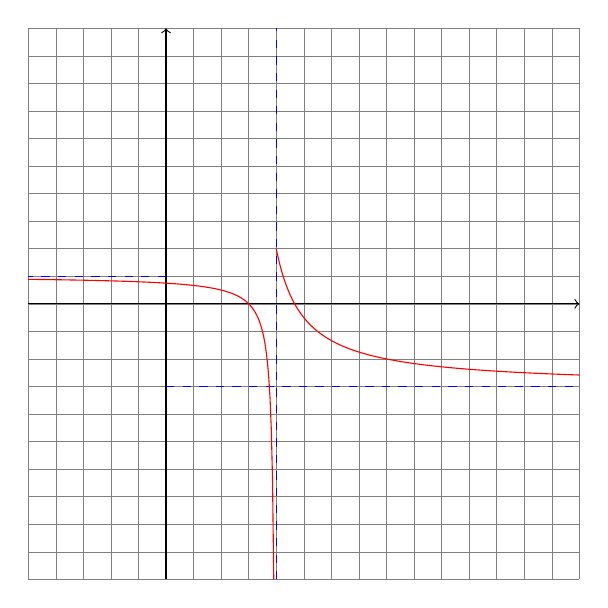
\begin{tikzpicture}[scale=0.35]
      \draw[gray,very thin] (-5,-10) grid (15,10);
      \draw[->] (-5,0)--(15,0);
      \draw[->] (0,-10)--(0,10);
      \draw[color=blue,dashed] (0,1)--(-5,1);
      \draw[color=blue,dashed] (0,-3)--(15,-3);
      \draw[color=blue,dashed] (4,-10)--(4,10);
      \draw[color=red,domain=-5:3.9090909,samples=200] plot(\x,{1+1/(\x-4)});
      % 1+1/(x-4)=-10 -> 1/(x-4)=-11 -> x-4=-1/11 -> x=4-1/11 -> x=3.9090...
      \draw[color=red,domain=4:15,samples=200] plot(\x,{-3+5/(\x-3)});
      % -3 + a/(4-3) = 2 -> a=5
    \end{tikzpicture}
    \\
    \mbox{(a) Asymptotes as Frame}
    &
    \mbox{(b) Graph Consistent with (a)}
    \end{array}$
    \caption{Asymptotes and Example of Graph Consistent with Asymptotes}
    \label{fig:asymptotes}
  \end{figure}
\item %2
  We first divide through by the highest power of $x$ in the
  denominator, namely $x^2$, to obtain
  \begin{displaymath}
    \lim_{x\to\infty} \frac{3x^2-8x+2}{x^2+6x-5}
    = \lim_{x\to\infty} \frac{3-\frac{8}{x}+\frac{2}{x^2}}{
      1+\frac{6}{x}-\frac{5}{x^2}}
  \end{displaymath}
  As $x\to\infty$, terms $8/x$, $2/x^2$, etc., tend to $0$ so we have
  \begin{displaymath}
    \lim_{x\to\infty} \frac{3x^2-8x+2}{x^2+6x-5}
    = \lim_{x\to\infty} \frac{3-\frac{8}{x}+\frac{2}{x^2}}{
      1+\frac{6}{x}-\frac{5}{x^2}}
    = \frac{3-0+0}{1+0-0} = 3
  \end{displaymath}
\item %3
  \begin{enumerate}
  \item %3a
    The highest power of $t$ in the denominator is $t^3$.  Dividing through,
    \begin{equation*}
      \lim_{t\to -\infty} \frac{t^2+2}{t^3+t^2-1}
      = \lim_{t\to -\infty} \frac{(1/t)+(2/t^3)}{1+(1/t)-(1/t^3)}
      = \frac{0+0}{1+0-0}
      = 0
    \end{equation*}
  \item %3b
    As usual, we divide through by the highest power of $x$ in the denominator.
    The highest power appears to be $x^2$, but since the $x^2$ is under a
    square root sign we use $\sqrt{x^2}$ instead:
    \begin{equation*}
      \lim_{x\to\infty} \frac{x+2}{\sqrt{9x^2+1}}
      = \lim_{x\to\infty} \frac{1+2/x}{\sqrt{9x^2+1}/x}
      = \lim_{x\to\infty} \frac{1+2/x}{\sqrt{(9x^2+1)/x^2}}
      = \lim_{x\to\infty} \frac{1+2/x}{\sqrt{9+1/x^2}}
      = \frac{1+0}{\sqrt{9+0}}
      = \frac{1}{3}
    \end{equation*}
  \item %3c
    The highest power of $x$ in the denominator is $x^3$.  We divide through
    by $x^3$:
    \begin{equation*}
      \lim_{x\to -\infty} \frac{\sqrt{9x^6-x}}{x^3+1}
      = \lim_{x\to -\infty} \frac{(9x^6-x)^{1/2}\cdot (1/x^3)}{1+(1/x^3)}
    \end{equation*}
    We need to bring $1/x^3$ into the square root.  We would like to write
    \begin{equation*}
      \frac{1}{x^3} = \left(\frac{1}{x^6}\right)^{1/2}
    \end{equation*}
    but in this case that is not quite correct.  Since $x\to -\infty$, we
    can assume that $x^3$ is negative, so $1/x^3$ is negative, but 
    $(1/x^6)^{1/2}$ is positive, so its sign is wrong.  Instead we must write
    \begin{equation*}
      \frac{1}{x^3} = -\left(\frac{1}{x^6}\right)^{1/2}
    \end{equation*}
    so our limit becomes
    \begin{multline*}
      \lim_{x\to -\infty} \frac{(9x^6-x)^{1/2}\cdot (1/x^3)}{1+(1/x^3)}
      = \lim_{x\to -\infty} \frac{(9x^6-x)^{1/2}\cdot -(1/x^6)^{1/2}}{1+(1/x^3)}
      \\
      = \lim_{x\to -\infty} \frac{-(9-1/x^5)^{1/2}}{1+(1/x^3)}
      = \frac{-(9-0)^{1/2}}{1+0} = -3
    \end{multline*}
    The correct answer is negative, not positive.
    % EJD: diagram
  \item %3d
    We know how to take infinite limits of fractions, so we try to convert
    the expression into a fraction.  Multiply and divide by the conjugate
    radical:
    \begin{multline*}
      \lim_{x\to -\infty} \left(x+\sqrt{x^2+2x}\right)
      = \lim_{x\to -\infty} \frac{\left(x+\sqrt{x^2+2x}\right)
        \left(x-\sqrt{x^2+2x}\right)}{x-\sqrt{x^2+2x}}
      \\
      = \lim_{x\to -\infty} \frac{x^2-(x^2+2x)}{x-\sqrt{x^2+2x}}
      = \lim_{x\to -\infty} \frac{-2x}{x-\sqrt{x^2+2x}}
    \end{multline*}
    Now divide through by the highest power of $x$ in the denominator.
    The $x^2$ in the denominator is under a square root sign so we think
    of it as $(x^2)^{1/2}\approx x$ so we divide through by $x$:
    \begin{equation*}
      \lim_{x\to -\infty} \frac{-2x}{x-\sqrt{x^2+2x}}
      = \lim_{x\to -\infty} \frac{-2}{1-\sqrt{x^2+2x}/x}
    \end{equation*}
    It is tempting to just write $x=\sqrt{x^2}$ to move it under the
    square root sign, but as with the previous problem, $x$ is negative
    while $\sqrt{x^2}$ is positive so we really have $x=-\sqrt{x^2}$ and
    we write
    \begin{multline*}
      \lim_{x\to -\infty} \frac{-2}{1-\sqrt{x^2+2x}/x}
      = \lim_{x\to -\infty} \frac{-2}{1+\sqrt{x^2+2x}/\sqrt{x^2}}
      = \lim_{x\to -\infty} \frac{-2}{1+\sqrt{(x^2+2x)/x^2}}
      \\
      = \lim_{x\to -\infty} \frac{-2}{1+\sqrt{1+2/x}}
      = \frac{-2}{1+\sqrt{1+0}}
      = -1
    \end{multline*}
    As with the previous problem, if you are not careful with this one you
    will get it wrong, in this case with
    a negative sign in front of the square root in the denominator
    which will lead to an infinite answer which is completely incorrect.
  \end{enumerate}
\item %4
  \begin{enumerate}
  \item %4a
    The horizontal asymptotes are found by evaluating
    \begin{displaymath}
      \lim_{x\to -\infty} \frac{3x-1}{x+2}
      = \lim_{x\to -\infty} \frac{3-\frac{1}{x}}{1+\frac{2}{x}}
      = 3, \qquad
      \lim_{x\to \infty} \frac{3x-1}{x+2}
      = \lim_{x\to \infty} \frac{3-\frac{1}{x}}{1+\frac{2}{x}}
      = 3
    \end{displaymath}
    giving $y=3$ as the only horizontal asymptote.  Candidates for the
    vertical asymptotes of a rational function are the roots of the
    denominator: $x+2=0 \implies x=-2$.  We check by evaluating the limits
    \begin{displaymath}
      \lim_{x\to -2^-} \frac{3x+1}{x+2} = \frac{7}{-0} = -\infty,
      \qquad
      \lim_{x\to -2^+} \frac{3x+1}{x+2} = \frac{7}{+0} = +\infty
    \end{displaymath}
    which shows that $x=-2$ is a vertical asymptote.  See
    Figure~\ref{fig:3asy}(a).
  \item %4b
    The horizontal asymptotes are found by evaluating
    \begin{displaymath}
      \lim_{x\to -\infty} \frac{x^2+x-6}{x^2-3x+2}
      = \lim_{x\to -\infty} \frac{1+\frac{1}{x}-\frac{6}{x^2}}{
        1 - \frac{3}{x} + \frac{2}{x^2}}
      = \frac{1+0-0}{1-0+0} = 1
    \end{displaymath}
    and
    \begin{displaymath}
      \lim_{x\to \infty} \frac{x^2+x-6}{x^2-3x+2}
      = \lim_{x\to \infty} \frac{1+\frac{1}{x}-\frac{6}{x^2}}{
        1 - \frac{3}{x} + \frac{2}{x^2}}
      = \frac{1+0-0}{1-0+0} = 1
    \end{displaymath}
    which give the only horizontal asymptote $y=1$.  The candidates
    for vertical asymptotes are $x$ values where the denominator of
    the rational function is zero: $x^2-3x+2=0 \implies (x-1)(x-2)=0$
    which gives candidates $x=1$, $x=2$.  To check whether they are
    actual vertical asymptotes we must evaluate the following limits:
    \begin{align*}
      \lim_{x\to 1^-} \frac{x^2+x-6}{x^2-3x+2}
      &= \lim_{x\to 1^-} \frac{(x+3)(x-2)}{(x-1)(x-2)}
        = \lim_{x\to 1^-} \frac{x+3}{x-1} = \frac{4}{-0} = -\infty \\
      \lim_{x\to 1^+} \frac{x^2+x-6}{x^2-3x+2}
      &= \lim_{x\to 1^+} \frac{(x+3)(x-2)}{(x-1)(x-2)}
        = \lim_{x\to 1^+} \frac{x+3}{x-1} = \frac{4}{+0} = +\infty \\
      \lim_{x\to 2^-} \frac{x^2+x-6}{x^2-3x+2}
      &= \lim_{x\to 2^-} \frac{(x+3)(x-2)}{(x-1)(x-2)}
        = \lim_{x\to 2^-} \frac{x+3}{x-1} = \frac{5}{1} = 5 \\
      \lim_{x\to 2^+} \frac{x^2+x-6}{x^2-3x+2}
      &= \lim_{x\to 2^+} \frac{(x+3)(x-2)}{(x-1)(x-2)}
        = \lim_{x\to 2^+} \frac{x+3}{x-1} = \frac{5}{1} = 5
    \end{align*}
    which show that $x=1$ is a vertical asymptote but $x=2$ is not.
    See Figure~\ref{fig:3asy}(b).
  \item %4c
    The horizontal asymptotes are found by evaluating
    \begin{displaymath}
      \lim_{x\to -\infty} \frac{1+2x^3}{x^3-x}
      = \lim_{x\to -\infty} \frac{\frac{1}{x^3}+2}{1-\frac{1}{x^2}}
      = \frac{0+2}{1-0} = 2
    \end{displaymath}
    and
    \begin{displaymath}
      \lim_{x\to \infty} \frac{1+2x^3}{x^3-x}
      = \lim_{x\to \infty} \frac{\frac{1}{x^3}+2}{1-\frac{1}{x^2}}
      = \frac{0+2}{1-0} = 2
    \end{displaymath}
    giving $y=2$ as the only horizontal asymptote.  The candidates for
    vertical asymptotes are $x$ values at which the denominator is
    $0$, in other words solutions to the equation $x^3-x=0$.
    Generally it is difficult to solve cubic equations, but this one
    can be solved by factoring:
    $x^3-x = x(x^2-1) = x(x-1)(x+1) = 0 \implies x=-1,0,1$.
    Evaluating left and right limits at each of those $x$ values gives
    \begin{align*}
      \lim_{x\to -1^-} \frac{1+2x^3}{x^3-x}
      &= \lim_{x\to -1^-} \frac{1+2x^3}{(x+1)x(x-1)}
        = \frac{1+2(-1)^3}{-0(-1)(-2)} = \frac{-1}{-0} = +\infty \\
      \lim_{x\to -1^+} \frac{1+2x^3}{x^3-x}
      &= \lim_{x\to -1^+} \frac{1+2x^3}{(x+1)x(x-1)}
        = \frac{1+2(-1)^3}{+0(-1)(-2)} = \frac{-1}{+0} = -\infty \\
      \lim_{x\to 0^-} \frac{1+2x^3}{x^3-x}
      &= \lim_{x\to 0^-} \frac{1+2x^3}{(x+1)x(x-1)}
        = \frac{1+2(0)^3}{(1)(-0)(-1)} = \frac{1}{+0} = +\infty \\
      \lim_{x\to 0^+} \frac{1+2x^3}{x^3-x}
      &= \lim_{x\to 0^+} \frac{1+2x^3}{(x+1)x(x-1)}
        = \frac{1+2(0)^3}{(1)(+0)(-1)} = \frac{1}{-0} = -\infty \\
      \lim_{x\to 1^-} \frac{1+2x^3}{x^3-x}
      &= \lim_{x\to 1^-} \frac{1+2x^3}{(x+1)x(x-1)}
        = \frac{1+2(1)^3}{(2)(1)(-0)} = \frac{3}{-0} = -\infty \\
      \lim_{x\to 1^+} \frac{1+2x^3}{x^3-x}
      &= \lim_{x\to 1^+} \frac{1+2x^3}{(x+1)x(x-1)}
        = \frac{1+2(1)^3}{(2)(1)(+0)} = \frac{3}{+0} = +\infty
    \end{align*}
    showing that there is a vertical asymptote at each of $x=-1,0,1$.
    See Figure~\ref{fig:3asy}(c).
  \end{enumerate}
  \begin{figure}[htbp]
    \centering
    $\begin{array}{c@{\hspace{0.25in}}c@{\hspace{0.25in}}c}
       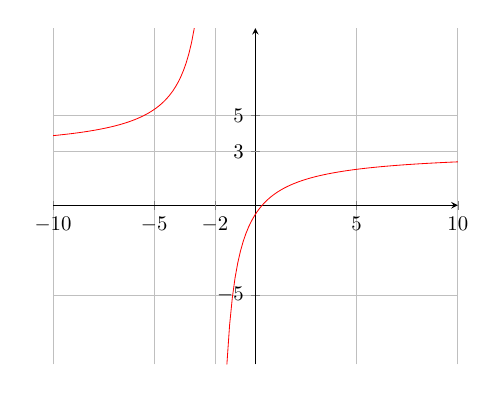
\begin{tikzpicture}[scale=0.75]
         \begin{axis}[domain=-10:10,samples=150,restrict y to domain=-10:10,
           extra x ticks=-2,
           extra y ticks=3,
           grid=both,axis lines=middle]
           \addplot[color=red] { (3*\x-1)/(\x+2) };           
         \end{axis}
       \end{tikzpicture}
     &
       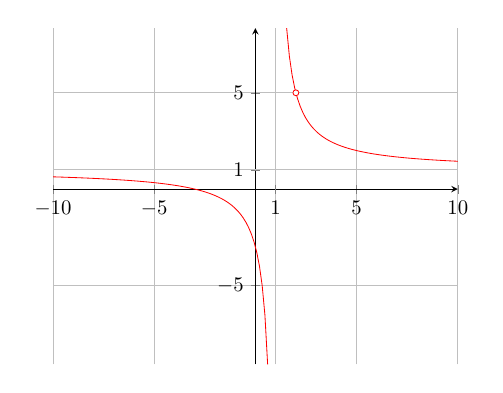
\begin{tikzpicture}[scale=0.75]
         \begin{axis}[domain=-10:10,samples=150,restrict y to domain=-10:10,
           extra x ticks=1,
           extra y ticks=1,
           grid=both,axis lines=middle]
           \addplot[color=red] { (\x*\x+\x-6)/(\x*\x-3*\x+2) };
           \node[draw=red,fill=white,circle,inner sep=1pt] at (axis cs:2,5) {};
         \end{axis}
       \end{tikzpicture}
    &
       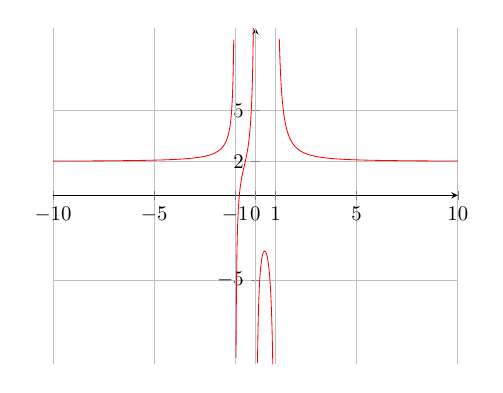
\begin{tikzpicture}[scale=0.75]
         \begin{axis}[domain=-10:10,samples=500,restrict y to domain=-10:10,
           extra x ticks={-1,0,1},
           extra y ticks=2,
           grid=both,axis lines=middle]
           \addplot[color=red,domain=-10:-1] { (1+2*\x*\x*\x)/(\x*\x*\x-\x) };
           \addplot[color=red,domain=-1:0] { (1+2*\x*\x*\x)/(\x*\x*\x-\x) }; 
           \addplot[color=red,domain=0:1] { (1+2*\x*\x*\x)/(\x*\x*\x-\x) };
           \addplot[color=red,domain=1:10] { (1+2*\x*\x*\x)/(\x*\x*\x-\x) };
         \end{axis}
       \end{tikzpicture}
    \\
    \mbox{(a) $y=\frac{3x+1}{x+2}$}
       &
    \mbox{(b) $y=\frac{x^2+x-6}{x^2-3x+2}$}
       &
    \mbox{(c) $y=\frac{1+2x^3}{x^3-x}$}
    \end{array}$
    \caption{Asymptotes for Three Functions}
    \label{fig:3asy}
  \end{figure}
\item %5 
  In Figure~\ref{fig:2exp} you can see the graph of the function
  plotted in two windows; in Figure~\ref{fig:2exp}(a) the $x$-axis
  goes from $0$ to $10$ and the $y$-axis goes from $0$ to $1$.  From
  that graph it appears that the function has a horizontal asymptote
  somewhere between $y=0.3$ and $y=0.4$.  In Figure~\ref{fig:2exp}(b)
  the $x$-axis is shifted to go from $90$ to $100$ and the $y$-axis is
  magnified to go from $0.3$ to $0.4$.  From that graph it seems
  likely that the horizontal asymptote rounded to two decimal points
  is $y=0.37$, so we conclude that the limit rounded to two decimal
  points is $0.37$.
  \begin{figure}[htbp]
    \centering
    $\begin{array}{c@{\hspace{0.25in}}c@{\hspace{0.25in}}c}
       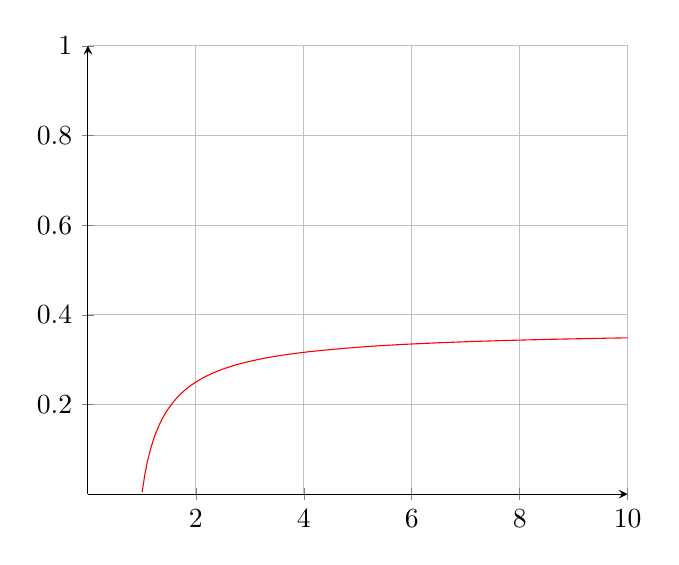
\begin{tikzpicture}[scale=1.0]
         \begin{axis}[domain=0:10,samples=200,ymin=0,ymax=1,
           restrict y to domain=-10:10,
           grid=both,axis lines=middle]
           \addplot[color=red] { (1-1/x)^x };
         \end{axis}
       \end{tikzpicture}
     &
       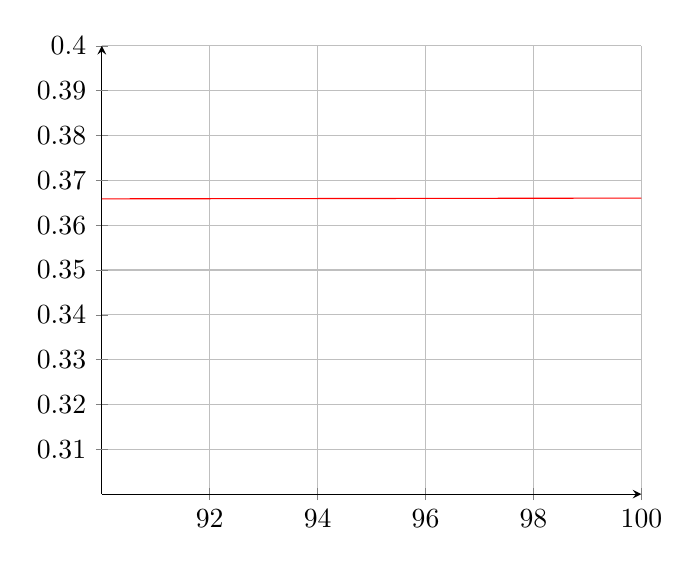
\begin{tikzpicture}[scale=1.0]
         \begin{axis}[domain=90:100,samples=3,ymin=0.3,ymax=0.4,
           restrict y to domain=0:1,
           extra y ticks={0.31,0.33,0.35,0.37,0.39},
           grid=both,axis lines=middle]
           \addplot[color=red,smooth] { (1-1/x)^x };
         \end{axis}
       \end{tikzpicture}
    \\
    \mbox{(a) Domain $0< x \le 10$}
       &
    \mbox{(b) Domain $90\le x \le 100$}
    \end{array}$
    \caption{Two Graphs of $f(x)=\left(1-\frac{1}{x}\right)^x$}
    \label{fig:2exp}
  \end{figure}

  The conclusion is supported by Table~\ref{tab:exp} where the
  function is calculated at successive powers of $10$.
  \begin{table}[htbp]
    \begin{center}
      \begin{tabular}{|r|l|l|l|}
        \hline
        \multicolumn{1}{|c|}{$x$}     
	         & \multicolumn{1}{|c|}{$1/x$}
		           & \multicolumn{1}{|c|}{$1-1/x$} 
			             & \multicolumn{1}{|c|}{$(1-1/x)^x$} \\
	\hline\hline
	$1$      & 1.0     & 0       & 0      \\
	\hline
	$10$     & 0.1     & 0.9     & 0.3486 \\
	\hline
	$100$    & 0.01    & 0.99    & 0.3660 \\
	\hline
	$1000$   & 0.001   & 0.999   & 0.3677 \\
	\hline
	$10000$  & 0.0001  & 0.9999  & 0.3679 \\
	\hline
	$100000$ & 0.00001 & 0.99999 & 0.3679 \\
	\hline
      \end{tabular}
    \end{center}
    \caption{Table of Values for $\left(1-\frac{1}{x}\right)^x$ to Four
      Decimal Points}
    \label{tab:exp}
  \end{table}
  In MATH 111 you will learn that the exact value of the limit is
  $1/e = 0.367879\ldots$.
\item %6
  In\label{prob:sqrtlim} order to calculate the limits, we divide
  through by the highest power of $x$ in the denominators.  For the
  limit as $x\to\infty$,
  \begin{displaymath}
    \lim_{x\to\infty} \frac{\sqrt{x^2+1}}{2x-3}
    = \lim_{x\to\infty} \frac{\sqrt{x^2+1}/x}{2-3/x}
    = \lim_{x\to\infty} \frac{\sqrt{(x^2+1)/x^2}}{2-3/x}
    = \lim_{x\to\infty} \frac{\sqrt{1+1/x^2}}{2-3/x}
    = \frac{\sqrt{1+0}}{2-0} = \frac{1}{2}
  \end{displaymath}
  where we square $x$ when we bring it under the square root.  On
  the other hand, for the limit as $x\to -\infty$,
  \begin{displaymath}
    \lim_{x\to -\infty} \frac{\sqrt{x^2+1}}{2x-3}
    = \lim_{x\to -\infty} \frac{\sqrt{x^2+1}/x}{2-3/x}
    = \lim_{x\to -\infty} \frac{-\sqrt{(x^2+1)/x^2}}{2-3/x}
    = \lim_{x\to -\infty} \frac{-\sqrt{1+1/x^2}}{2-3/x}
    = -\frac{\sqrt{1+0}}{2-0} = -\frac{1}{2}
  \end{displaymath}
  Note the appearance of the negative sign in the second step which
  may at first be puzzling.  This phenomenon, which may occur when
  taking limits at infinity of functions involving roots, is unlike
  what happens with ordinary rational functions which always have
  equal limits as $x\to \pm\infty$.  The negative sign appears because
  $x$ is negative in the limit $x\to -\infty$, but $\sqrt{x^2}$ is
  positive.  For equality in this case we must write $x=-\sqrt{x^2}$.
  See Figure~\ref{fig:sqrtlim}.
  \begin{figure}[htbp]
    \centering
    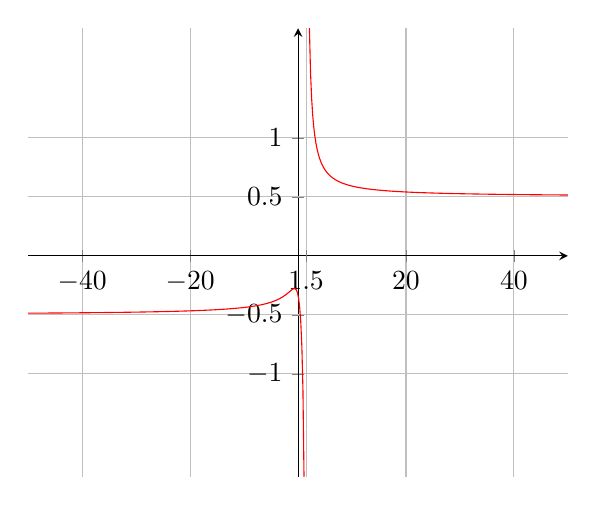
\begin{tikzpicture}
      \begin{axis}[domain=-50:50,restrict y to domain=-2:2,
        extra x ticks=1.5,
        extra y ticks={-0.5,0.5},
        grid=both, axis lines=middle,
        samples=500]
        \addplot[color=red] { sqrt(x^2+1)/(2*x-3) };
      \end{axis}
    \end{tikzpicture}
    \caption{Graph of $\ds y=\frac{\sqrt{x^2+1}}{2x-3}$}
    \label{fig:sqrtlim}
  \end{figure}
\item %7
  We will find a rational function satisfying the given conditions.
  The denominator of the function should contain factors $x+2$ and
  $x-3$; $(x+2)(x-3)=x^2-x-6$ is the simplest choice.  In order for
  the function to have a horizontal asymptote the highest power of $x$
  in the numerator must match the highest power of $x$ in the
  denominator; $x^2$ is the simplest choice for the numerator.  (We
  must also ensure that neither $x+2$ nor $x-3$ is a factor of the
  numerator.)  Finally, to scale the horizontal asymptote to $5/2$
  from its current value of $1$, we just multiply the function by
  $5/2$ to obtain
  \begin{displaymath}
    f(x) = \frac{5x^2}{2x^2-2-12}
  \end{displaymath}
  You should check that the resulting function satisfies the
  conditions of the problem.  You should also try to find other
  answers to the problem.
\item %8
  This question is like Example~11 in Section~3.4 of the textbook.
  The $y$-intercept is
  \begin{displaymath}
    y=f(0) = 0^2(0+2)^3(1-0) = 0
  \end{displaymath}
  so $(0,0)$ is a point on the graph.  The $x$-intercepts are roots of
  the equation
  \begin{displaymath}
    f(x)=0 \implies x^2(x+2)^3(1-x)=0 \implies x=-2,0,1
  \end{displaymath}
  so $(-2,0)$, $(0,0)$, and $(1,0)$ are points on the graph.  In
  addition, a careful analysis shows that the function does not change
  sign at $x=0$ because the $x^2$ factor has an even exponent, but the
  function does change sign at $x=-2$ and $x=1$ because of the odd
  exponents in the factors $(x+2)^3$ and $(1-x)^1$.  As $x\to\infty$,
  \begin{displaymath}
    \lim_{x\to\infty} x^2(x+2)^3(1-x) = -\infty
  \end{displaymath}
  because for large positive $x$ the $x^2$ and $(x+2)^3$ are positive,
  while $(1-x)$ is negative.  Similarly, as $x\to -\infty$,
  \begin{displaymath}
    \lim_{x\to -\infty} x^2(x+2)^3(1-x) = -\infty
  \end{displaymath}
  because for large negative $x$ the $x^2$ term is positive, the
  $(x+2)^3$ term is negative, and the $(1-x)$ term is positive.
  Putting all the information together, your graph should resemble
  Figure~\ref{fig:sixdeg}.
  \begin{figure}[htbp]
    \centering
    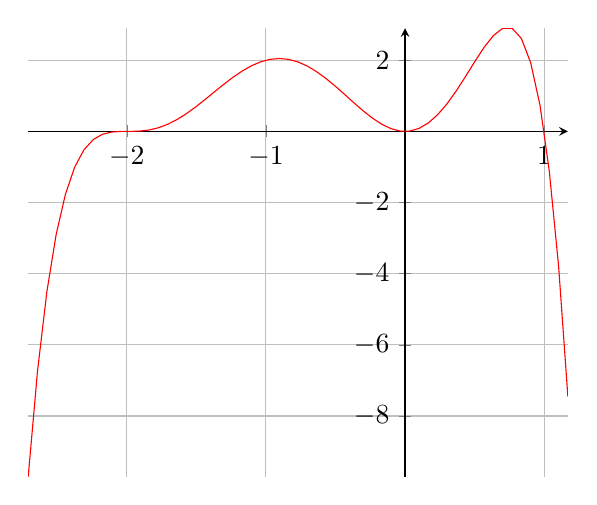
\begin{tikzpicture}
      \begin{axis}[domain=-10:10,restrict y to domain=-10:10,
        %extra x ticks=1.5,
        %extra y ticks={-0.5,0.5},
        grid=both, axis lines=middle,
        samples=300]
        \addplot[color=red] { x^2*(x+2)^3*(1-x) };
      \end{axis}
    \end{tikzpicture}
    \caption{Graph of $\ds y=x^2(x+2)^3(1-x)$}
    \label{fig:sixdeg}
  \end{figure}
% \item %10
%   This is an application of the Squeeze Theorem for infinite limits.
%   We have
%   \begin{align*}
%     \lim_{x\to\infty} \frac{4x-1}{x} 
%     &= \lim_{x\to\infty} \frac{4-1/x}{1}
%     = \frac{4-0}{1} = 4
%     \\
%     \lim_{x\to\infty} \frac{4x^2+3x}{x^2} 
%     &= \lim_{x\to\infty} \frac{4+3/x}{1}
%     = \frac{4+0}{1} = 4
%   \end{align*}
%   Since the two limits are equal, the limit for $f(x)$ is squeezed between
%   the two outer limits to obtain
%   \begin{equation*}
%     \lim_{x\to\infty} f(x) = 4
%   \end{equation*}
% \item\label{prob:funknown} %11
%   We don't know what $f$ is, but we only need $f'$ to construct our usual
%   table for intervals of increase/decrease.  The critical numbers are at the
%   zeros of $f'$, namely $x=-1$, $x=3$, and $x=6$, which gives us 
%   Table~\ref{tab:funknown}.
%   \begin{table}[htbp]
%     \centering
%     \begin{tabular}{|c|c|c|c|c|c|}
%       \hline
%       Interval       & $(x+1)^2$ & $(x-3)^5$ & $(x-6)^4$ & $f'(x)$ & $f$
%       \\
%       \hline\hline
%       $-\infty<x<-1$ & $+$       & $-$       & $+$       & $-$     & decreasing
%       \\
%       \hline
%       $x=-1$         & $0$       & $-$       & $+$       & $0$     & stationary
%       \\
%       \hline
%       $-1<x<3$       & $+$       & $-$       & $+$       & $-$     & decreasing
%       \\
%       \hline
%       $x=3$          & $+$       & $0$       & $+$       & $0$     & stationary
%       \\
%       \hline
%       $3<x<6$        & $+$       & $+$       & $+$       & $+$     & increasing
%       \\
%       \hline
%       $x=6$          & $+$       & $+$       & $0$       & $0$     & stationary
%       \\
%       \hline
%       $6<x<\infty$   & $+$       & $+$       & $+$       & $+$     & increasing
%       \\
%       \hline
%     \end{tabular}
%     \caption{Intervals of Increase/Decrease for problem~\ref{prob:funknown}}
%     \label{tab:funknown}
%   \end{table}
%   Note that the minus signs in the $(x+1)^2$ and $(x-6)^4$ columns have
%   flipped to plus signs because the power is an even number in both cases.
%   We conclude that $f$ is increasing on just
%   the intervals $(3,6)$ and $(6,\infty)$.
%   % EJD: diagram
% \item %12
%   % EJD: later
%   We'll do this later.
% \item %13
%   The derivatives are
%   \begin{align*}
%     y' &= \frac{(1+x^2)-(1+x)(2x)}{(1+x^2)^2} = (1-2x-x^2)(1+x^2)^{-2} \\
%     y'' &= (-2-2x)(1+x^2)^{-2} + (1-2x-x^2)(-2)(1+x^2)^{-3}(2x)
%   \end{align*}
%   Simplifying the second derivative,
%   \begin{align*}
%     y'' &= -2(1+x^2)^{-3} \left[(x+1)(1+x^2) +(2x)(1-2x-x^2)\right]
%     \\
%     &= -2(1+x^2)^{-3} \left[x^3+x^2+x+1-2x^3-4x^2+2x\right]
%     \\
%     &= 2 (1+x^2)^{-3} (x^3+3x^2-3x-1)
%   \end{align*}
%   We need to further factor $y''$.  We guess roots which divide the constant
%   term in the cubic $-x^3-3x^2+3x+1$, namely $1$, so our guesses for roots
%   are $\pm 1$.  The root $x=1$ works so we can pull out a factor $(x-1)$
%   by polynomial division or otherwise:
%   \begin{align*}
%     y'' = 2(1+x^2)^{-3} (x-1)(x^2+4x+1)
%   \end{align*}
%   We complete factoring by using the quadratic formula to get the roots
%   $x=-2-\sqrt{3}$ and $x=-2+\sqrt{3}$, so we can write
%   \begin{align*}
%     y'' = 2(1+x^2)^{-3} (x-(-2-\sqrt{3}))(x-(-2+\sqrt{3}))(x-1)
%   \end{align*}
%   The potential inflection numbers are the numbers $x$ where $y''$ is 
%   undefined (nowhere, since the denominator $(1+x^2)^3$ is never $0$) and
%   where $y''=0$, namely $x=-2-\sqrt{3}$, $x=-2+\sqrt{3}$ and $x=1$.  You
%   can make a table for the sign of $y''$ if you wish, but since each of
%   the factors in the numerator is not to an even power, the sign of $y''$
%   will change across each of those potential inflection numbers, so the
%   concavity will change at each of those potential inflection numbers, so
%   each of those potential inflection numbers is an actual inflection number.
%   (Make a table if you are confused by the above discussion.)

%   To find the actual inflection points, we evaluate $y$ at each of the
%   inflection numbers:
%   \begin{align*}
%     y(-2-\sqrt{3}) = \frac{1+-2-\sqrt{3}}{1+(-2-\sqrt{3})^2}
%     = \frac{-1-\sqrt{3}}{1+4+4\sqrt{3}+3}
%     = \frac{-1-\sqrt{3}}{8+4\sqrt{3}}
%     = -\frac{1}{4} \frac{1+\sqrt{3}}{2+\sqrt{3}}
%   \end{align*}
%   It will be convenient to rationalize the denominator by multiplying
%   through by the conjugate of the denominator:
%   \begin{equation*}
%     y(-2-\sqrt{3}) 
%     = -\frac{1}{4}\frac{(1+\sqrt{3})(2-\sqrt{3})}{(2+\sqrt{3})(2-\sqrt{3})}
%     = -\frac{1}{4} \frac{-1+\sqrt{3}}{1}
%     = \frac{1}{4} (1-\sqrt{3})
%   \end{equation*}
%   Similarly (just changing some of the plus signs to minus signs in the above
%   two calculations) we obtain
%   \begin{equation*}
%     y(-2+\sqrt{3})
%     = \frac{1}{4} (1+\sqrt{3})
%   \end{equation*}
%   and obviously $y(1)=(1+1)/(1+1)=1$.  So the three points of inflection
%   are
%   \begin{equation*}
%     \mbox{$(-2-\sqrt{3},1/4-(1/4)\sqrt{3})$, $(-2+\sqrt{3},1/4+(1/4)\sqrt{3})$,
%       and $(1,1)$}
%   \end{equation*}
%   There are various ways to show that three points lie on a straight line,
%   the most straightforward of which is to find the line through two of
%   the points and show that the third point lies on that line.  We find
%   the line through the first two inflection points.  The slope of the
%   line is
%   \begin{equation*}
%     m = \frac{y_2-y_1}{x_2-x_1}
%     = \frac{(1/4)(1+\sqrt{3})-(1/4)(1-\sqrt{3})}{(-2+\sqrt{3})-(-2-\sqrt{3})}
%     = \frac{1}{4} \frac{2\sqrt{3}}{2\sqrt{3}} = \frac{1}{4}
%   \end{equation*}
%   So one way to write the equation of the line through the first two 
%   inflection points is
%   \begin{equation*}
%     y-y_1 = m(x-x_1) \implies
%     y-\frac{1}{4}(1-\sqrt{3}) = \frac{1}{4} (x-(-2-\sqrt{3}))
%   \end{equation*}
%   Obviously the second inflection point lies on that line, so we only need
%   to check whether the third inflection point $(1,1)$ also lies on it.
%   The left hand side of the equation for the line is
%   \begin{equation*}
%     1-\frac{1}{4}(1-\sqrt{3}) = \frac{3}{4} + \frac{1}{4}\sqrt{3}
%   \end{equation*}
%   while the right hand side is
%   \begin{equation*}
%     \frac{1}{4} (1-(-2-\sqrt{3}) = \frac{1}{4} (3+\sqrt{3})
%     = \frac{3}{4} + \frac{1}{4} \sqrt{3}
%   \end{equation*}
%   Since the LHS and the RHS agree, $(1,1)$ also lies on the line, so all
%   three points lie on the same straight line.
% \item %14
%   % EJD: later
%   We'll do this later.
\end{enumerate}
\end{document}


